% Generated by scripts/make_explanation_figures.py from experiment_0013 (do not edit by hand).
% Model: COVER $-$conflict
\documentclass[tikz,border=3pt]{standalone}
\usepackage[T1]{fontenc}
\usepackage[utf8]{inputenc}
\usepackage{newtxtext,newtxmath}
\usetikzlibrary{positioning,arrows.meta,calc}

\definecolor{neural}{HTML}{2F6DB5}
\definecolor{neuralbg}{HTML}{E8F0FA}
\definecolor{logic}{HTML}{2E8B57}
\definecolor{logicbg}{HTML}{E6F4EC}
\definecolor{relneg}{HTML}{C0392B}

\tikzset{
  tok/.style={draw=neural!80, fill=white, rounded corners=1.5pt, inner sep=1.6pt, font=\scriptsize,
              minimum height=4mm, anchor=base},
  htok/.style={tok, fill=neural!12},
  stok/.style={tok, draw=black!25, text=black!45},
  aedge/.style={line width=#1, draw=logic},
  cedge/.style={line width=#1, draw=relneg},
  ledge/.style={line width=#1, draw=neural, densely dashed},
  rlab/.style={font=\tiny, fill=white, inner sep=0.6pt},
}
\newcommand{\bars}[4]{%
  \fill[logic]  (#1-0.17,0.05) rectangle ++(0.15,{0.8*#2});
  \fill[relneg] (#1+0.02,0.05) rectangle ++(0.15,{0.8*#3});
  \node[font=\tiny, anchor=north] at (#1-0.095,0.03) {$s$};
  \node[font=\tiny, anchor=north] at (#1+0.095,0.03) {$c$};
  \node[font=\tiny, anchor=north] at (#1,-0.22) {$#2\,/\,#3$};
  \node[font=\tiny, anchor=north, text=black!60] at (#1,-0.47) {$\omega{=}#4$};
}
\newcommand{\sbar}[3]{%
  \fill[logic]  (#1-0.075,0.05) rectangle ++(0.15,{0.8*#2});
  \node[font=\tiny, anchor=north] at (#1,0.03) {$s$};
  \node[font=\tiny, anchor=north] at (#1,-0.22) {$#2$};
  \node[font=\tiny, anchor=north, text=black!60] at (#1,-0.47) {$\omega{=}#3$};
}
\providecommand{\Pcov}{P_{\mathrm{cov}}}
\providecommand{\Pnc}{P_{\neg\mathrm{conf}}}
\providecommand{\E}{\textsc{e}}
\providecommand{\N}{\textsc{n}}
\providecommand{\C}{\textsc{c}}

\begin{document}
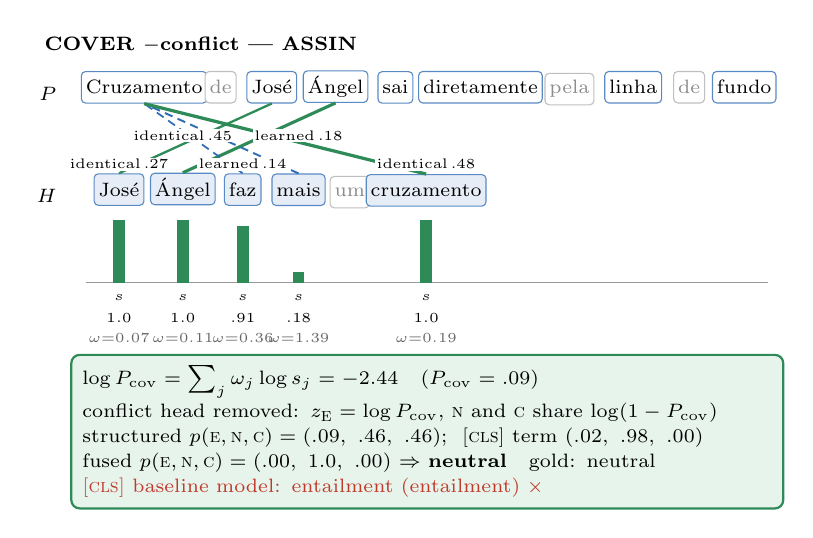
\begin{tikzpicture}
\begin{scope}[xshift=0.00cm]
\node[font=\scriptsize\itshape, anchor=east] at (-0.35,2.45) {$P$};
\node[font=\scriptsize\itshape, anchor=east] at (-0.35,1.15) {$H$};
\node[tok] (p1) at (0.64,2.45) {Cruzamento};
\node[stok] (pw1) at (1.61,2.45) {de};
\node[tok] (p4) at (2.26,2.45) {José};
\node[tok] (p5) at (3.07,2.45) {Ángel};
\node[tok] (p8) at (3.83,2.45) {sai};
\node[tok] (p9) at (4.91,2.45) {diretamente};
\node[stok] (pw6) at (6.04,2.45) {pela};
\node[tok] (p11) at (6.85,2.45) {linha};
\node[stok] (pw8) at (7.56,2.45) {de};
\node[tok] (p13) at (8.26,2.45) {fundo};
\node[htok] (h16) at (0.32,1.15) {José};
\node[htok] (h17) at (1.13,1.15) {Ángel};
\node[htok] (h20) at (1.89,1.15) {faz};
\node[htok] (h21) at (2.60,1.15) {mais};
\node[stok] (hw4) at (3.25,1.15) {um};
\node[htok] (h23) at (4.22,1.15) {cruzamento};
\draw[aedge=0.83pt] (h16.north) -- (p4.south);
\draw[aedge=1.13pt] (h17.north) -- (p5.south);
\draw[ledge=0.63pt] (h20.north) -- (p1.south);
\draw[ledge=0.70pt] (h21.north) -- (p1.south);
\draw[aedge=1.17pt] (h23.north) -- (p1.south);
\node[rlab, anchor=south] at (0.32,1.47) {identical\,.27};
\node[rlab, anchor=south] at (1.13,1.83) {identical\,.45};
\node[rlab, anchor=south] at (1.89,1.47) {learned\,.14};
\node[rlab, anchor=south] at (2.60,1.83) {learned\,.18};
\node[rlab, anchor=south] at (4.22,1.47) {identical\,.48};
\draw[black!40] (-0.1,0.05) -- (8.56,0.05);
\sbar{0.32}{1.0}{0.07}
\sbar{1.13}{1.0}{0.11}
\sbar{1.89}{.91}{0.36}
\sbar{2.60}{.18}{1.39}
\sbar{4.22}{1.0}{0.19}
\end{scope}
\node[draw=logic, fill=logicbg, rounded corners=3pt, line width=0.8pt, font=\scriptsize, align=left, anchor=north west, text width=8.76cm, inner sep=4pt] (agg) at (-0.3,-0.85) {%
  $\log\Pcov=\sum_j\omega_j\log s_j=-2.44$\quad($\Pcov=.09$)\\[1pt]conflict head removed: $z_\E=\log\Pcov$, \N{} and \C{} share $\log(1-\Pcov)$\\[1pt]structured $p(\E,\N,\C)=(.09,\ .46,\ .46)$;\ \ \textsc{[cls]} term $(.02,\ .98,\ .00)$\\[1pt]fused $p(\E,\N,\C)=(.00,\ 1.0,\ .00)$ $\Rightarrow$ \textbf{neutral}\quad gold: neutral\\[1pt]\textcolor{relneg}{\textsc{[cls]} baseline model: entailment (entailment) \texttimes}};
\node[font=\scriptsize\bfseries, anchor=south west] at (-0.75,2.85) {COVER $-$conflict --- ASSIN};
\end{tikzpicture}
\end{document}
